\documentclass[11pt]{article}

% ---------- Packages ----------
\usepackage[margin=1in]{geometry}
\usepackage[T1]{fontenc}
\usepackage[utf8]{inputenc}
\usepackage{lmodern}
\usepackage{setspace}
\usepackage{hyperref}
\usepackage{graphicx}
\usepackage{booktabs}
\usepackage{enumitem}
\usepackage{caption}
\usepackage{subcaption}
\usepackage{xcolor}
\usepackage{listings}
\usepackage{amsmath,amssymb}
\usepackage{cleveref}

% ---------- Metadata ----------
\title{17-614: Project Write-up: Modeling \textit{Presto} (Ride Sharing App)}
\author{Team \#12 \quad | \quad Iris Huang, Viren Dodia, Ziqin Shen, Ray Xue}
\date{\today}

% ---------- Document ----------
\begin{document}
\maketitle

\newpage

\section{Task 1: Structural Modeling}
\label{sec:task1}

\subsection{Object Model Diagram}
\label{sec:object-model}

\begin{figure}[h]
  \centering
  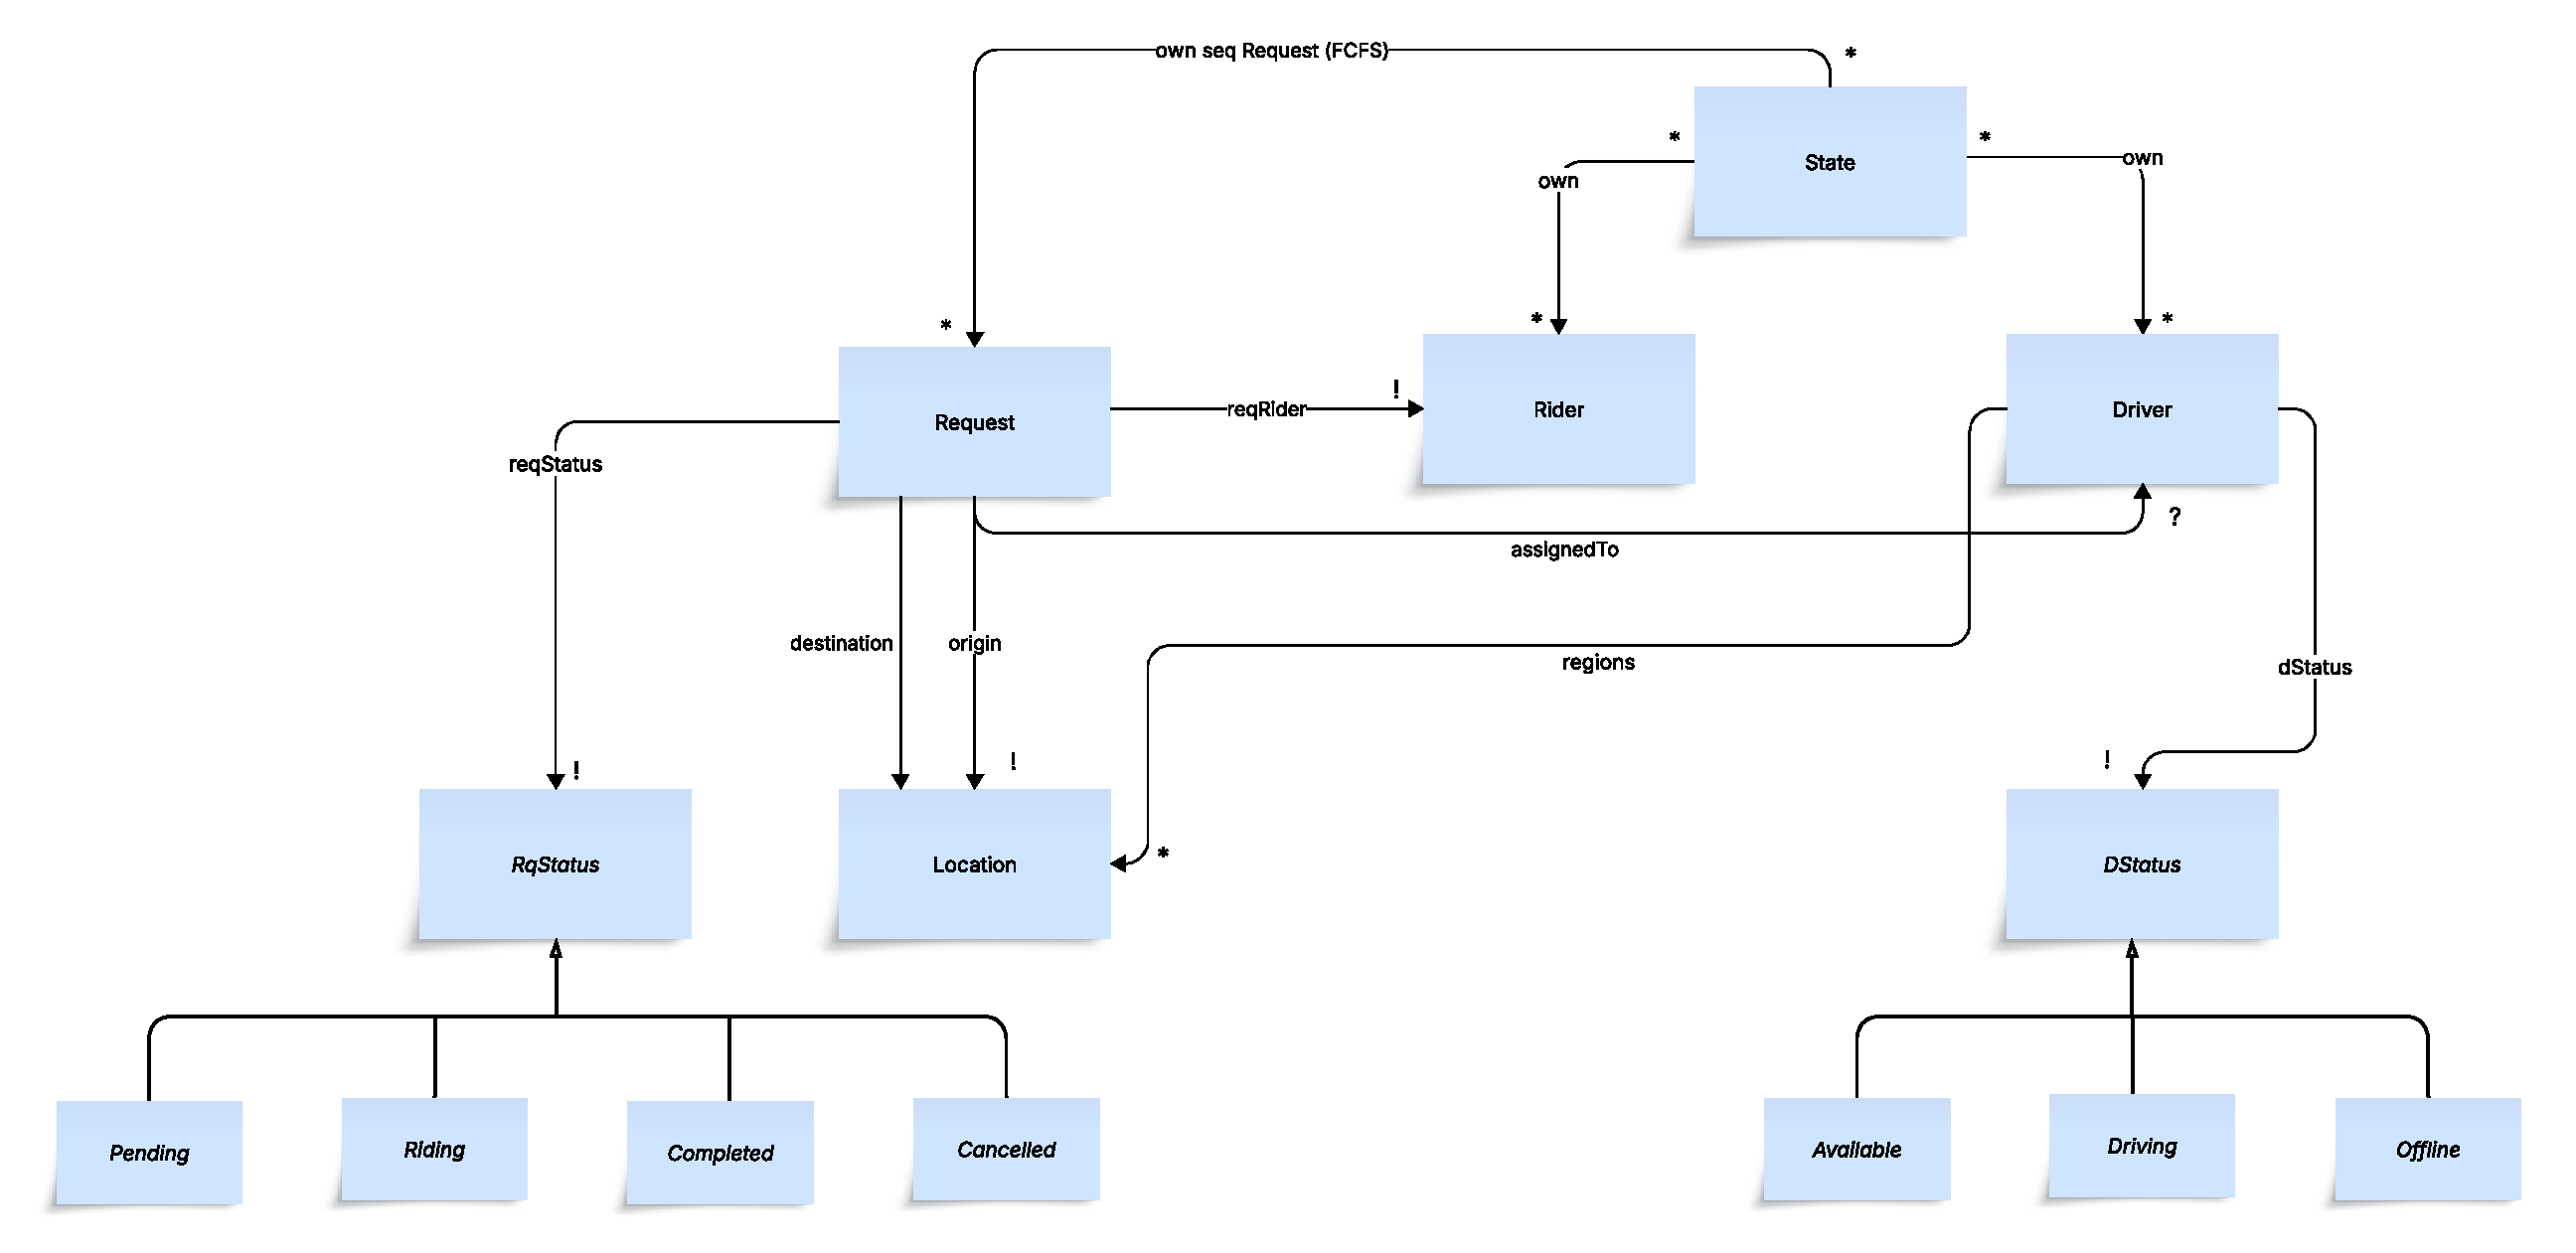
\includegraphics[width=1.00\linewidth]{figs/object-model.pdf}
  \caption{Object model of the \textit{Presto} system.}
\end{figure}

\subsection{Invariants Discovered During Modeling}

During Alloy modeling of \textit{Presto}, we identified several invariants that ensure consistency of the system state:

\begin{itemize}[leftmargin=1.5em]
  \item \textbf{One active request per rider}: Each rider can have at most one request that is either \texttt{Pending} or \texttt{Riding}.
  \item \textbf{Driver exclusivity}: Each driver can serve at most one request at a time. A driver is in the \texttt{Driving} state if and only if they are assigned to exactly one active request.
  \item \textbf{Assignment consistency}: A request in \texttt{Riding} must have exactly one assigned driver. Requests in \texttt{Pending}, \texttt{Completed}, or \texttt{Cancelled} must have no assigned driver.
  \item \textbf{Queue well-formedness}: The set of requests in the \texttt{Pending} state must exactly equal the elements of the \texttt{pendingQ} sequence (with no duplicates).
  \item \textbf{Origin-destination sanity}: For realism, each request must have distinct origin and destination.
\end{itemize}
These invariants capture both explicit rules in the specification and implicit requirements necessary to preserve logical correctness.

\subsection{Model Validation Strategy}

Our validation strategy for the Alloy model involved:
\begin{itemize}[leftmargin=1.5em]
  \item \textbf{Operation preservation checks}: We wrote assertions ensuring that the four core operations (\texttt{request}, \texttt{cancel}, \texttt{match}, and \texttt{complete}) preserve the system invariants across state transitions.
  \item \textbf{Visualization of states}: Using \texttt{run} commands, we generated concrete states, such as an empty system, one pending request, and one riding request. These helped confirm intuitive behavior.
  \item \textbf{Counterexample analysis}: If Alloy produced a counterexample, we refined the model (e.g., corrected scoping errors or missing conditions) until the invariants held.
  \item \textbf{Cross-checking with the spec}: Each invariant and operation was traced back to requirements in the Presto specification to ensure coverage.
\end{itemize}
In addition, we developed a suite of \textbf{positive and negative test predicates} 
to exercise the model further. Positive tests (e.g., \texttt{test\_MultiplePending}, 
\texttt{test\_MultipleConcurrentRides}) confirmed that realistic states were satisfiable, 
while negative tests (e.g., \texttt{test\_RidingRequestInPendingQueue}, 
\texttt{test\_AvailableDriverIsAssigned}, \texttt{test\_DuplicateRequestInQueue}) 
demonstrated that invalid states were impossible under our invariants. 
Running these tests under scopes of 4–7 atoms with exactly one \texttt{State} 
reinforced our confidence that the model was both correct and complete.

\subsection{Scopes for Checking Assertions}

For invariant preservation checks, we used scopes of 6–7 objects with exactly one State and up to 6 sequence elements. 
This bound was sufficient because:
\begin{itemize}[leftmargin=1.5em]
  \item It allowed us to explore diverse combinations of Riders, Drivers, and Requests while keeping the analysis tractable.
  \item Larger scopes (beyond 7) did not uncover new counterexamples, suggesting our invariants are robust.
  \item These bounds match the project’s guidance for balancing coverage with solver performance.
\end{itemize}

\section{Task 2: Concurrency with FSP/LTSA}
\label{sec:task2}

\subsection{Process Structure Diagram}

\label{sec:process-structure}
\begin{figure}[h]
  \centering
  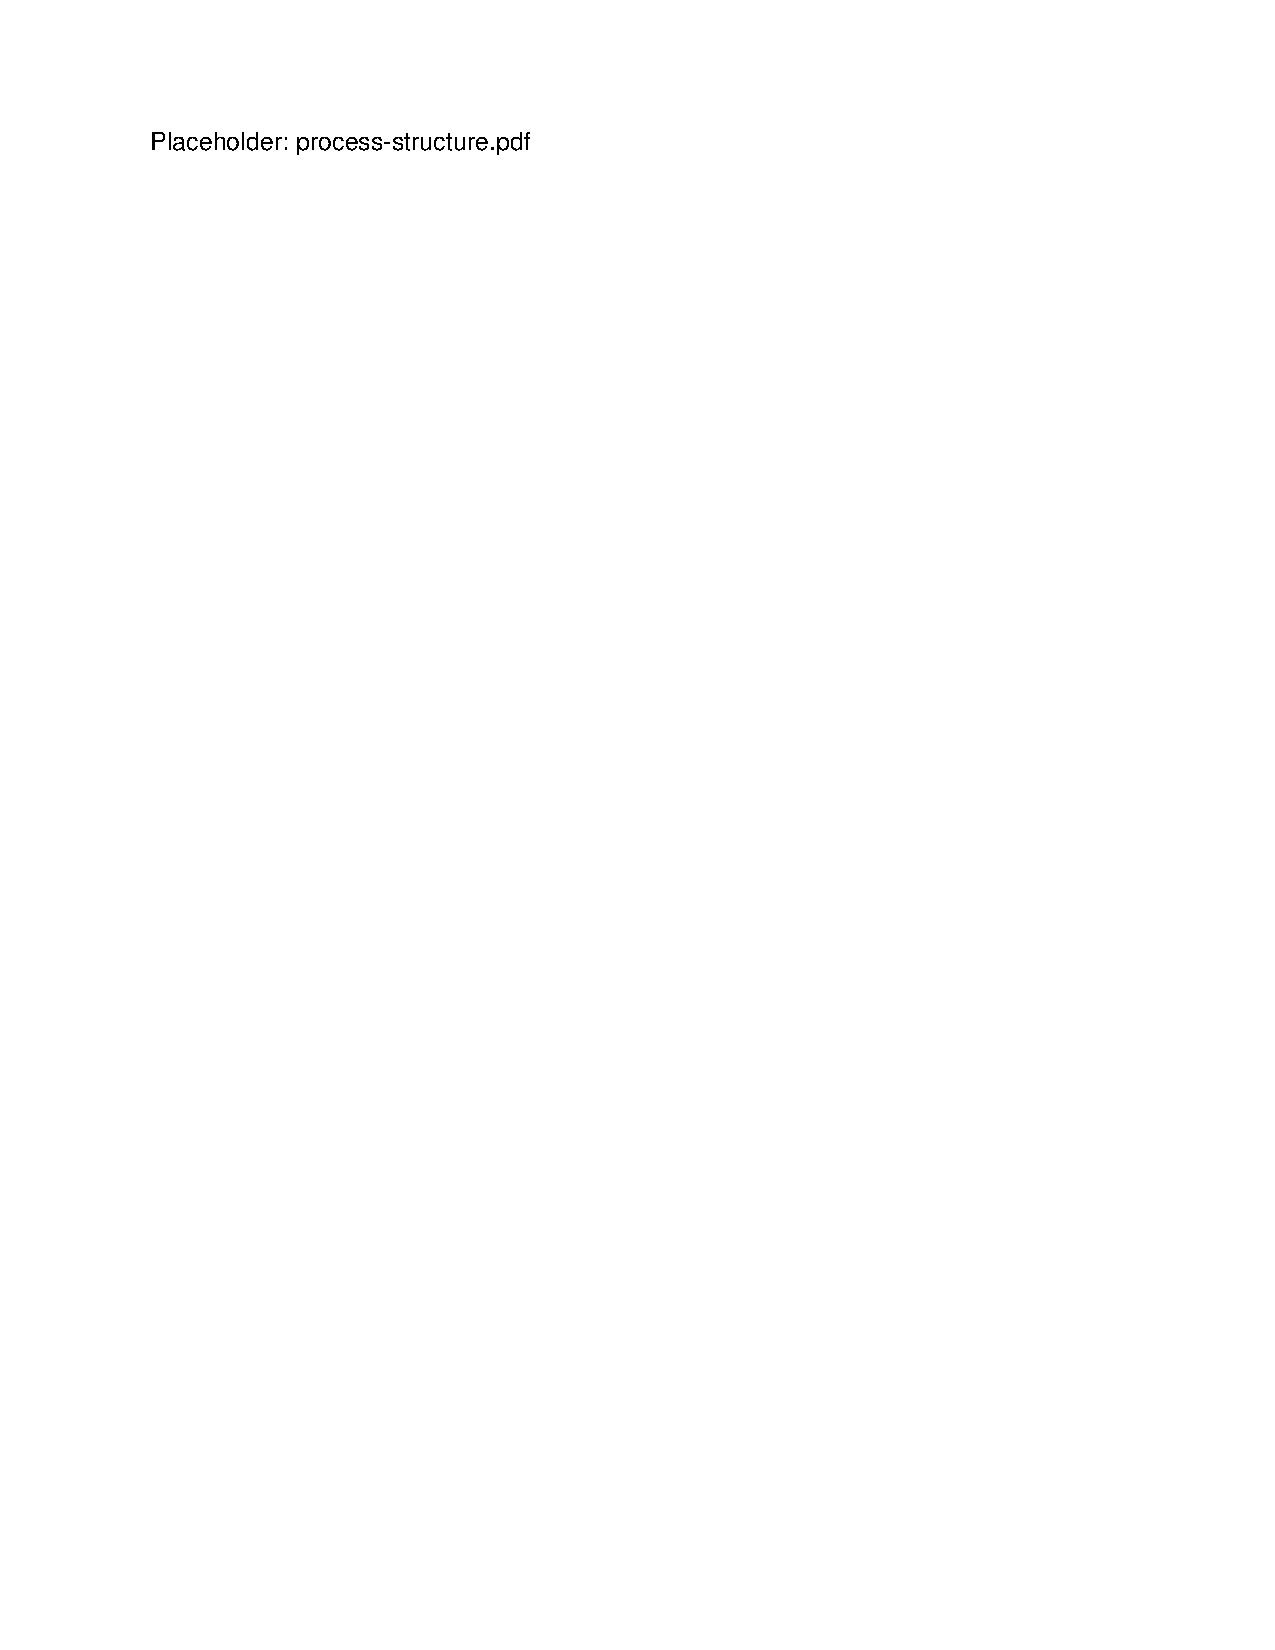
\includegraphics[width=0.50\linewidth]{figs/process-structure.pdf}
  \caption{Process Structure diagram for the FSP model.}
\end{figure}

\subsection{Protocol Design}

% Your response 

\subsection{Details Abstracted from Task 1}

% Your response 

\subsection{Details Added Beyond Task 1}

% Your response 

\section{Task 3: Reflection}
\label{sec:task3}

\subsection{Alloy: Strengths and Weaknesses}

\textbf{Strengths:}
\begin{itemize}[leftmargin=1.5em]
  \item Naturally suited for modeling structural constraints and invariants.
  \item Immediate visualization of counterexamples, which aids debugging.
  \item Compact and expressive syntax for relational properties.
\end{itemize}
\textbf{Weaknesses:}
\begin{itemize}[leftmargin=1.5em]
  \item Not designed to capture concurrency or event ordering explicitly.
  \item Large scopes can cause performance issues.
  \item Expressing temporal behaviors (e.g., eventuality) requires workarounds.
\end{itemize}

\subsection{FSP/LTSA: Strengths and Weaknesses}

% Your response 

\subsection{Other Aspects of Ride Sharing}

While our models capture the core protocol, real-world ride sharing involves additional aspects:
\begin{itemize}[leftmargin=1.5em]
  \item \textbf{Pricing and payment}: Fare calculation, dynamic pricing, and payment handling.
  \item \textbf{Trust and reputation}: Ratings, cancellation penalties, and fraud prevention.
  \item \textbf{Geographic constraints}: Real-world routing, travel times, and multi-region rides.
  \item \textbf{System resilience}: Handling driver disconnections, rider no-shows, or sudden surges.
\end{itemize}

\end{document}